\documentclass{standalone}

\usepackage{tikz}
\usetikzlibrary{angles,quotes}
\usepackage{amsmath,amssymb,amsfonts}

\usepackage{pgfplots}
\definecolor{darkgreen}{rgb}{0.0, 0.42, 0.24}
\definecolor{amethyst}{rgb}{0.6, 0.4, 0.8}

\pgfplotsset{compat=newest}
\pgfplotsset{every axis/.append style={
                     tick label style={font=\footnotesize},
                 }}


\begin{document}
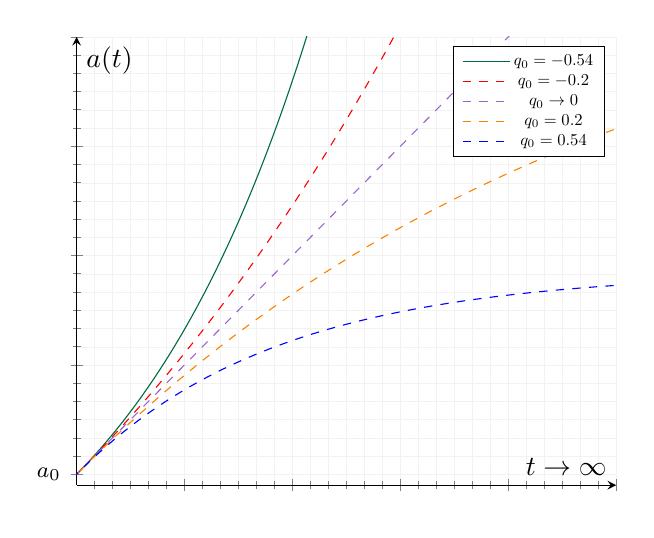
\begin{tikzpicture}
 \begin{axis}[axis lines =center,xmin=0,xmax=5,ymin=0.9,ymax=5,
 grid=both,
    grid style={line width=.1pt, draw=gray!10},
    major grid style={line width=.2pt,draw=gray!10},
     minor tick num=5,
 xticklabels=false,
 ytick={1,2,3,4,5},
 yticklabels={$a_0$},
 xlabel=$t\rightarrow\infty$,ylabel=$a(t)$,
 legend style={nodes={scale=0.6, transform shape}}]
 
    \addplot[color=darkgreen,samples=300]{-(1/0.54)*(1-0.54-e^(0.54*x))};
     \addplot[color=red,samples=300,dashed]{-(1/0.2)*(1-0.2-e^(0.2*x))};
      \addplot[color=amethyst,samples=300,dashed]{x+1};
       \addplot[color=orange,samples=300,dashed]{(1/0.2)*(1+0.2-e^(-0.2*x))};
        \addplot[color=blue,samples=300,dashed]{(1/0.54)*(1+0.54-e^(-0.54*x))};
        
        \addlegendentry{$q_0=-0.54$};
        \addlegendentry{$q_0=-0.2$};
        \addlegendentry{$q_0\rightarrow0$};
        \addlegendentry{$q_0=0.2$};
        \addlegendentry{$q_0=0.54$};
 \end{axis}

\end{tikzpicture}
\end{document}